\chapter{Implementation}
\label{ch:whatYouDid}

\com{
\todo[inline]{Choose your own chapter title to describe this}

\todo[inline]{What have you done? How did you do it? What design decisions did you make? How did what you did help you to meet your goals?}



Describe the engineering-related contents (preferably with models) and the research methodology and methods that are used in the degree project.

Give a theoretical description of the scientific or engineering methodology are you going to use and why have you chosen this method. What other methods did you consider and why did you reject them.

In this chapter, you describe what engineering-related and scientific skills you are going to apply, such as modeling, analyzing, developing, and evaluating engineering-related and scientific content. The choice of these methods should be appropriate for the problem . Additionally, you should be consciousness of aspects relating to society and ethics (if applicable). The choices should also reflect your goals and what you (or someone else) should be able to do as a result of your solution - which could not be done well before you started.

The purpose of this chapter is to provide an overview of the research method
used in this thesis. Section~\ref{sec:researchProcess} describes the research
process. Section~\ref{sec:researchParadigm} details the research
paradigm. Section~\ref{sec:dataCollection} focuses on the data collection
techniques used for this research. Section~\ref{sec:experimentalDesign}
describes the experimental design. Section~\ref{sec:assessingReliability}
explains the techniques used to evaluate the reliability and validity of the
data collected. Section~\ref{sec:plannedDataAnalysis} describes the method
used for the data analysis. Finally, Section~\ref{sec:evaluationFramework}
describes the framework selected to evaluate xxx.

}
DRAFT

\noindent
The platform adopted, \gls{HRP}, has been improved starting from its configuration and sensors' drivers.



\section{Hardware Configuration}
\label{sec:system}

\noindent
\gls{HRP} that holds the sensors and the raspberry pi, also proving the measurements of the wheel encoders and of the embedded GPS receiver.
Computer to guide the automower and make him move according to the desired path, also at the end the automower was free to run its random path and use the algorithm implemented to stay inside the boundaries.

\com{
\begin{figure}[!ht]
  \begin{center}
    \includegraphics[width=0.5\textwidth]{Images/4-Done/}
  \end{center}
  \caption{Hardware}
  \label{fig:hardware}
\end{figure}
}



\subsection{Sensors}
\label{ssec:sens}
\noindent
The following set of sensors are available for fusion using the \gls{AEKF} defined in \ref{ch:methods}.

\subsubsection{Wheel Encoder}
\noindent
It is included in the motor of the wheel of the \gls{ALM}, inside the Motor Kit shown in \ref{fig:wheelenc}.
Measure the wheel displacement and provide \gls{WO}, as explained in \ref{ch:methods}.

\begin{figure}[!ht]
	\begin{center}
		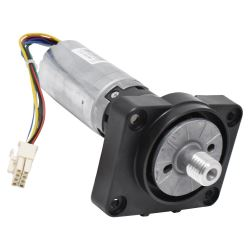
\includegraphics[width=0.5\textwidth]{Images/4-Methods/MotorEnc.jpeg}
	\end{center}
	\caption{Motor Kit Automower 450X }
	\label{fig:wheelenc}
\end{figure}

The performances have been examined and are available below.
\missingfigure[]{Wheel Encoder Performances}

They are mounted in the wheel axis on both wheels.

\subsubsection{Global Navigation Satellite System}

\noindent Measure the satellite positions to estimate its absolute position global values in the global coordinate frame.

Different \glspl{GNSS} are available.
A \gls{GPS} receiver is embedded in the \gls{HRP}, shown in \ref{fig:autogps}.
Moreover, two additional \gls{GPS} receivers has been added, shown in \ref{fig:phigps}.

\begin{figure}[!ht]
\begin{center}
	\begin{subfigure}{.5\textwidth}
		\centering
		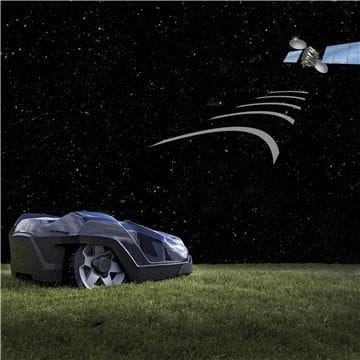
\includegraphics[width=0.75\textwidth]{Images/4-Methods/AutomowerGPS.jpeg}
		\caption{Automower 450X GPS}
		\label{fig:autogps}
	\end{subfigure}%
	\begin{subfigure}{.5\textwidth}
		\centering
		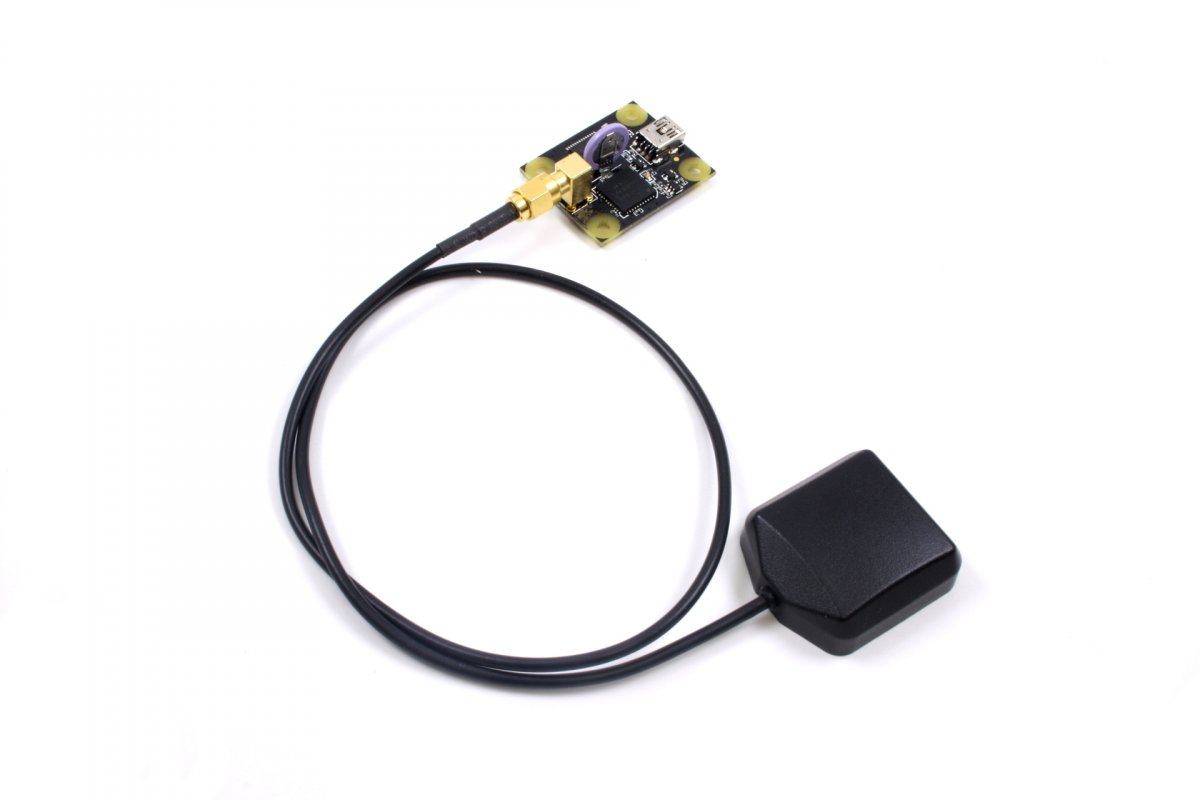
\includegraphics[width=0.75\textwidth]{Images/4-Methods/1040_0B_Alt2.jpg}
		\caption{PhidgetGPS ID: 1040\_0B}
		\label{fig:phigps}
	\end{subfigure}
	\caption{\glspl{GNSS} receivers adopted}
	\label{fig:gpssenso}
\end{center}
\end{figure}

The performances have been examined and are available below.
\missingfigure{GNSS Performances}


It is mounted in front, at coordinate x,y,z with orientation theta with respect to the robot coordinate frame.

\subsubsection{Inertial Measurement Unit}

\noindent Measure the angular velocity, acceleration, and magnetic fields in the three orthogonal axis.

This PhidgetSpatial Precision 3/3/3 High Resolution, shown in \ref{fig:spatial}, has a 3-axis accelerometer, gyroscope and compass with high resolution readings at low magnitudes.

\begin{figure}[!ht]
	\begin{center}
		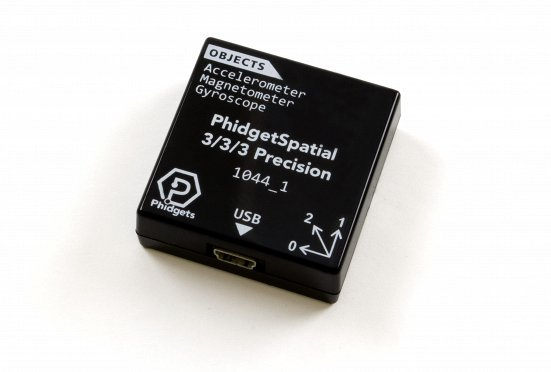
\includegraphics[width=0.5\textwidth]{Images/4-Methods/1044_1B.jpg}
	\end{center}
	\caption{PhidgetSpatial Precision 3/3/3 High Resolution - ID: 1044\_1B}
	\label{fig:spatial}
\end{figure}


The performances have been examined and are available below.
\missingfigure[]{IMU Performances}

It is mounted in front, at coordinate x,y,z with orientation theta with respect to the robot coordinate frame.

\subsubsection{RGB-D Camera}

\noindent Measure the displacement of the camera \gls{F2F} and provide \gls{VO}.
The device that is used is the RealSense D435 shown in Figure.
It provides \gls{RGBD} images, i.e. both \gls{RGB} and depth information.

"The Intel® RealSense™ depth camera D435 is a stereo solution, offering quality depth for a variety of applications. It's wide field of view is perfect for applications such as robotics or augmented and virtual reality, where seeing as much of the scene as possible is vitally important."

\begin{figure}[!ht]
	%\textbf{Investigating Simultaneous Localization and Mapping for AGV systems}
	\begin{center}
		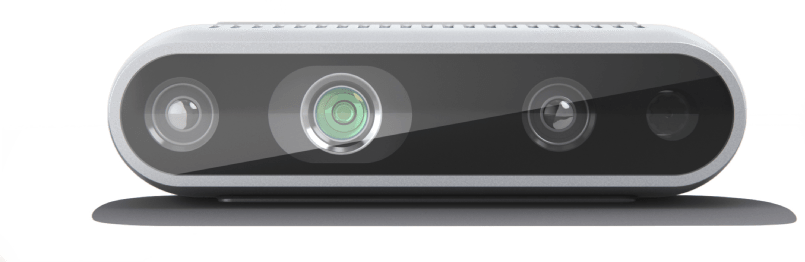
\includegraphics[width=0.75\textwidth]{Images/4-Methods/d435i-1.png}
	\end{center}
	\caption{Intel® RealSense™ depth camera D435}
	\label{fig:d435}
\end{figure}

It is mounted in front, at coordinate x,y,z with orientation theta with respect to the robot coordinate frame.

\subsection{Devices}
\label{ssec:dev}
\noindent
Raspberry Pi 4 to guide the automower, to gather information about the topics of ROS, and to communicate them to the personal computer used to gather them.

\subsubsection{Raspberry Pi 4}
\noindent
On this device, most of the embedded devices will be attached.
The \gls{HRP}, the \glspl{IMU}, and the camera.

\begin{figure}[!ht]
	\begin{center}
		\begin{subfigure}[b]{.45\textwidth}
			\begin{center}
				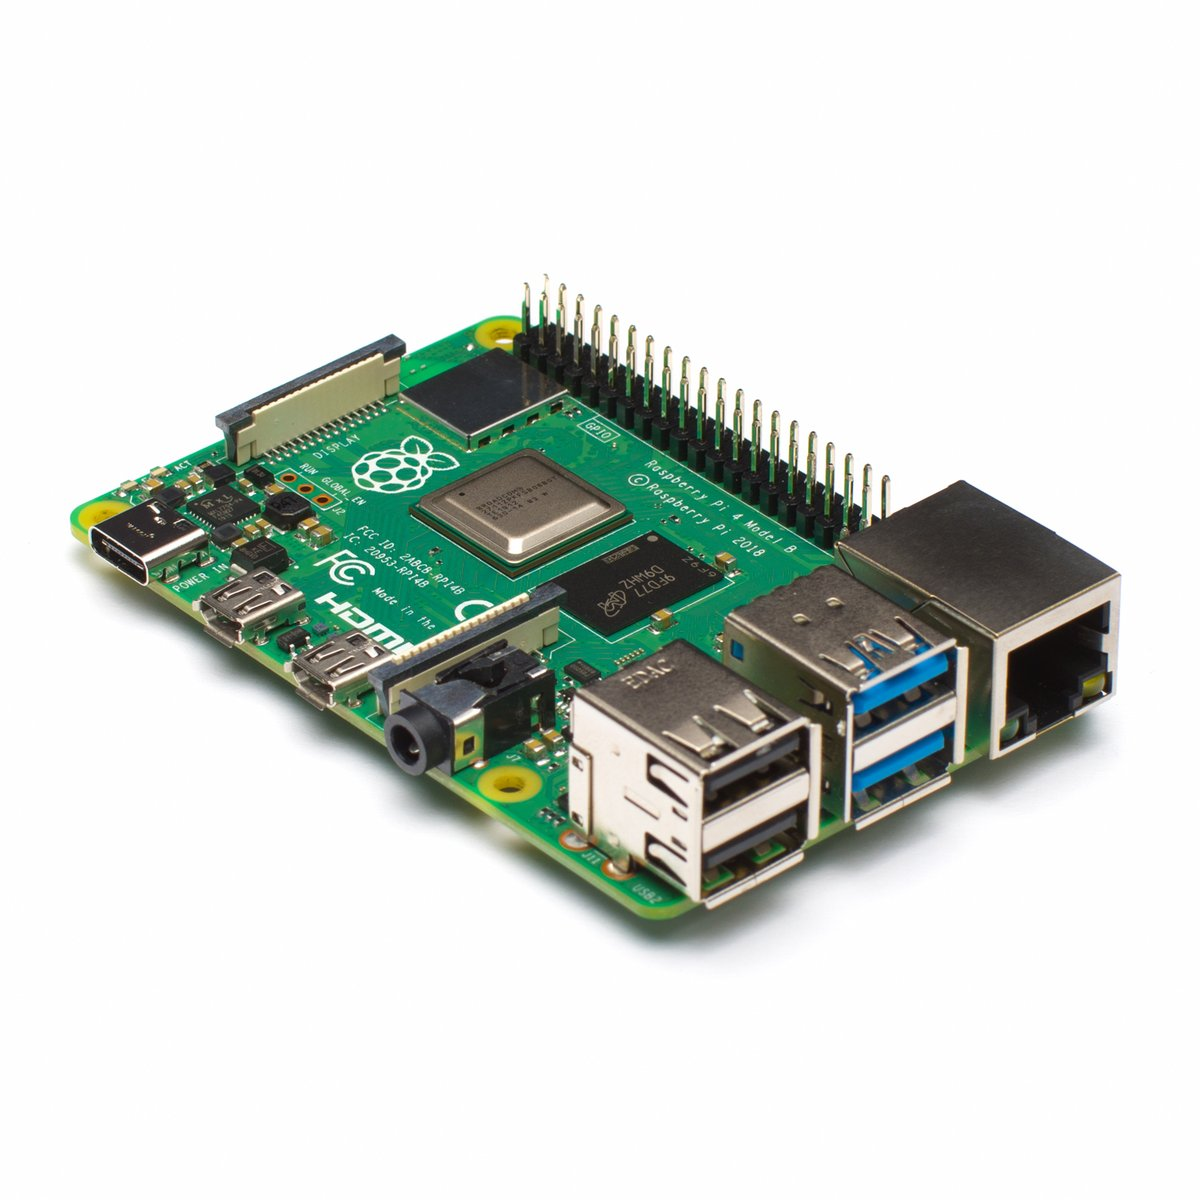
\includegraphics[width=0.75\textwidth]{Images/4-Methods/RPi4.jpg}
			\end{center}
			\caption{Raspberry Pi 4 Model B}
			\label{fig:rpi4Im}
		\end{subfigure}%
		\begin{subfigure}[b]{.45\textwidth}
			\begin{center}
				\begin{tikzpicture}[font=\small,thick]
					\node[draw, text centered, fill=white!30,
					align=center,
					minimum width=3cm,
					minimum height=1cm,
					] (block0) { Raspberry Pi 4};

					\node[draw,text centered,fill=white!30,rounded corners,
					right=of block0, align=center,
					minimum width=2.5cm,
					minimum height=1cm,
					] (block1) { \gls{HRP} Automower };

					\node[draw,text centered,fill=yellow!30,rounded corners,
					above=of block1,
					align=center,
					minimum width=2.5cm,
					minimum height=1cm,
					] (block2) { Phidget \glspl{IMU}};

					\node[draw,text centered,fill=green!30,rounded corners,
					below=of block1,
					align=center,
					minimum width=2.5cm,
					minimum height=1cm,
					] (block3) { Camera};

					% Arrows
					\draw[latex-] (block0) edge (block1);
					\draw[latex-] (block0) edge (block2);
					\draw[latex-] (block0) edge (block3);
				\end{tikzpicture}
				\caption[Caption]{Raspberry Pi 4 configuration \centering}
			\end{center}
			\label{fig:RPi4Conf}
		\end{subfigure}
		\caption{Raspberry Pi 4}
		\label{fig:RPi4}
	\end{center}
\end{figure}


\subsubsection{Raspberry Pi 3}
\noindent
On this device, running Ubuntu 20, the Phidgets GPS sensors will be attached.


\begin{figure}[!ht]
	\begin{center}
		\begin{subfigure}[b]{.5\textwidth}
			\begin{center}
				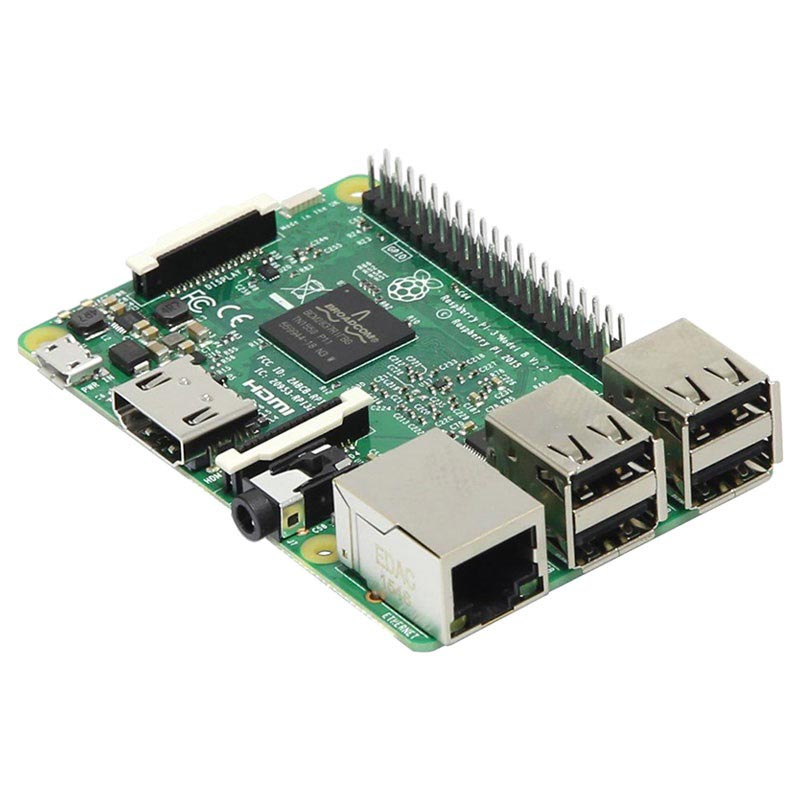
\includegraphics[width=0.33\textwidth]{Images/4-Methods/RPi3.jpg}
			\end{center}
			\caption{Raspberry Pi 3 Model B}
			\label{fig:rpi3Im}
		\end{subfigure}%
		\begin{subfigure}[b]{.5\textwidth}
			\begin{center}
				\begin{tikzpicture}[font=\small,thick]
					\node[draw, text centered, fill=white!30,
					align=center,
					minimum width=3cm,
					minimum height=1cm,
					] (block0) { Raspberry Pi 3};

					\node[draw,text centered,fill=cyan!30,rounded corners,
					right=of block0, align=center,
					minimum width=2.5cm,
					minimum height=1cm,
					] (block1) { Phidget \glspl{GPS} };
					% Arrows
					\draw[latex-] (block0) edge (block1);
				\end{tikzpicture}
				\caption[Caption]{Raspberry Pi 3 configuration \centering}
			\end{center}
			\label{fig:RPi3Conf}
		\end{subfigure}
		\caption{Raspberry Pi 3}
		\label{fig:RPi3}
	\end{center}
\end{figure}

\section{Software Configuration}
\noindent
C++ and Python development to work with the ROS framework.

Network establishment to communicate wirelessly between Raspberry Pi and computer.

Communication through hotspot




\subsubsection{Robotic Operating System Framework}
\label{ssec:ros}
\noindent \Gls{ROS}\cite{288} is an open-source framework, and not an actual operating system, widely adopted for building software used to control robotic systems.
\Gls{ROS} works both with C++ and Python programmed scripts, allowing for developers with different backgrounds to develop upon it.


For these nodes to cooperate, they are connected by a middle-layer structure based on a network of topics or services, following a blackboard architecture of data sharing.
It provides a graph-like structure were each program, described as node, can both publish and subscribe messages among the created and available topics.

Topics can be seen as variables which are used for streaming communication and share information between nodes.
A \Gls{ROS} node publishes a specific message through a topic and every other node can subscribe to that topic and receive all the messages posted to it.
A \Gls{ROS} system, to behave as expected, needs a master process which has the task of matching publishers and subscribers to their related topics.

These topics can be generated by sensors, actuators, planners, controllers of different kind and made available using this structure of topics, similar to a blackboard architecture.
Each topic is defined by a specific message type which specifies its content in order to standardise its usage among applications and to simplify communication between nodes.
Messages definition can be customised and they are stored inside the \Gls{ROS} package, defining the data sent within the topic which will use that definition.

Figure \ref{fig:ros-topic} shows an example of a \Gls{ROS} graph where two subscriber nodes receive the messages posted on the topic by a publisher node.

\begin{figure}[!ht]
	%\textbf{Investigating Simultaneous Localization and Mapping for AGV systems}
	\begin{center}
		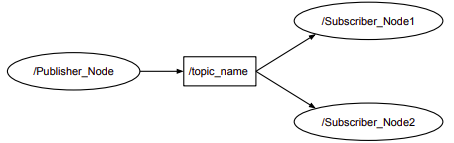
\includegraphics[width=0.75\textwidth]{Images/2-Background/ROSTopic-2021-04-22 10-51-37.png}
	\end{center}
	\caption{\Gls{ROS} topics architecture}% for information sharing\cite{palsson_investigating_2017}}
	\label{fig:ros-topic}
\end{figure}

The aspect of localisation is important for the robotics field, to understand where the robot is located with respect to the rest of the world, but also to know how the sensors are positioned with respect to the robot in which they are installed.
It is of prominent importance to be aware of the different pose of the connected sensors before fusing their information, as the measurements of each sensors are related to their specific coordinate frame.

Before performing sensors fusion, every different frames of the sensors need to be transformed into the base frame of the robot which they are measuring to be sure about that the measurements refers to the same coordinate frame.

\Gls{ROS} uses the TF\cite{6556373} library to provide the tools needed to work with coordinate frames and to deal with their related transformation.
It allows for the definition of each sensor rigid body transform to specify their related position with respect to the robot, and then the library will deal with all the other transformations by publishing messages regarding to the rotational and translational relations between frames.
Commonly used frames are odom and base\_link.. The odom frame has the origin at the initial position $P_{odom}$ of the robot and it is used to keep track of its moving behaviour. The base\_link frame is rigidly attached to the robot base $P_{base}$ and it is used to define the frames of its attached components.

Executing automower\_hrp.launch


\subsubsection{Velocity Control}
\label{sec:control}
\noindent A script is used to control the vehicle setting the desired robot velocities: $v$ and $\omega$.
In this way it is possible to command the \gls{ALM} to follow a trajectory.

Executing hrp\_teleop.launch


\subsubsection{Launching the sensors}
\noindent The sensors are launched using the following scripts.

Executing imus\_basic.launch

Executing gps.launch

Executing rs\_camera.launch

Executing VO package



\subsubsection{Launching the sensor fusion}
\noindent A script is used to control the vehicle setting the desired robot velocities: $v$ and $\omega$.
In this way it is possible to command the \gls{ALM} to follow a trajectory.

Executing EKF

\subsubsection{Launching the mapping update}
\noindent
Executing map generation and update




\cleardoublepage
%\clearpage
